\documentclass[14pt,a4paper]{scrreprt}

\usepackage{cmap}
\usepackage[T1]{fontenc} 
\usepackage[utf8]{inputenc}
\usepackage[english,russian]{babel}

\usepackage{caption}
\usepackage{subcaption}

\usepackage{float}

\usepackage{enumitem}

\usepackage{graphicx}
\usepackage{multirow}


\usepackage{pgfplots}
\pgfplotsset{compat=newest}
\usepgfplotslibrary{units}

\usepackage{longtable}

\usepackage{caption}
\captionsetup{labelsep=endash}
\captionsetup[figure]{name={Рисунок}}
\captionsetup[subtable]{labelformat=simple}
\captionsetup[subfigure]{labelformat=simple}
\renewcommand{\thesubtable}{\text{Таблица }\arabic{chapter}\text{.}\arabic{table}\text{.}\arabic{subtable}\text{ --}}
\renewcommand{\thesubfigure}{\text{Рисунок }\arabic{chapter}\text{.}\arabic{figure}\text{.}\arabic{subfigure}\text{ --}}


\usepackage{textcomp}

\usepackage{amsmath}
\usepackage{amsfonts}
\usepackage{array}

\usepackage{geometry}
\geometry{left=30mm}
\geometry{right=15mm}
\geometry{top=20mm}
\geometry{bottom=20mm}
\geometry{foot=1.7cm}

\usepackage{titlesec}
\titleformat{\section}
{\normalsize\bfseries}
{\thesection}
{1em}{}
\titlespacing*{\chapter}{0pt}{-30pt}{8pt}
\titlespacing*{\section}{\parindent}{*4}{*4}
\titlespacing*{\subsection}{\parindent}{*4}{*4}

% Маркировка для списков
\def\labelitemi{$\circ$}
\def\labelitemii{$*$}


\usepackage{setspace}
\onehalfspacing % Полуторный интервал

\frenchspacing
\usepackage{indentfirst} % Красная строка

\usepackage{titlesec}
\usepackage{xcolor}
% Названия глав
\titleformat{\section}{\normalsize\textmd}{\thesection}{1em}{}

\definecolor{gray35}{gray}{0.35}

\newcommand{\hsp}{\hspace{20pt}} % длина линии в 20pt

\titleformat{\chapter}[hang]{\Huge}{\textcolor{gray35}{\thechapter.}\hsp}{0pt}{\Huge\textmd}

\titleformat{\section}{\Large}{\textcolor{gray35}\thesection}{20pt}{\Large\textmd}
\titleformat{\subsection}{\Large}{\thesubsection}{20pt}{\Large\textmd}
\titleformat{\subsubsection}{\normalfont\textmd}{}{0pt}{}

% Настройки введения

\addtocontents{toc}{\setcounter{tocdepth}{2}}
\addtocontents{toc}{\setcounter{secnumdepth}{1}}

\usepackage{tocloft,lipsum,pgffor}

\addtocontents{toc}{~\hfill\textnormal{Страница}\par}

\renewcommand{\cftpartfont}{\normalfont\textmd}

\addto\captionsrussian{\renewcommand{\contentsname}{Содержание}}
\renewcommand{\cfttoctitlefont}{\Huge\textmd}

\renewcommand{\cftchapfont}{\normalfont\normalsize}
\renewcommand{\cftsecfont}{\normalfont\normalsize}
\renewcommand{\cftsubsecfont}{\normalfont\normalsize}
\renewcommand{\cftsubsubsecfont}{\normalfont\normalsize}

\renewcommand{\cftchapleader}{\cftdotfill{\cftdotsep}}

\usepackage{listings}
\usepackage{xcolor}

\usepackage[pdftex]{hyperref} % Гиперссылки
\hypersetup{hidelinks}

% Листинги 
\usepackage{listings}

\definecolor{darkgray}{gray}{0.15}

\definecolor{teal}{rgb}{0.25,0.88,0.73}
\definecolor{gray}{rgb}{0.5,0.5,0.5}
\definecolor{b-red}{rgb}{0.88,0.25,0.41}
\definecolor{royal-blue}{rgb}{0.25,0.41,0.88}

\usepackage{listings}
\lstset{
	aboveskip=3mm,
	belowskip=3mm,
	frame=tb,
	frame=single,
	basicstyle=\footnotesize\ttfamily,
	numberstyle=\tiny\color{gray},
	keywordstyle=\color{royal-blue},
	commentstyle=\color{gray35},
	stringstyle=\color{b-red},
	numbers=left,
	numbersep=5pt,
	numberstyle=\tiny,
	showstringspaces=false, 
	captionpos=t,
	tabsize=4,
	language=C
}

% какой то сложный кусок со стак эксчейндж для квадратных скобок
\makeatletter
\newenvironment{sqcases}{%
	\matrix@check\sqcases\env@sqcases
}{%
	\endarray\right.%
}
\def\env@sqcases{%
	\let\@ifnextchar\new@ifnextchar
	\left\lbrack
	\def\arraystretch{1.2}%
	\array{@{}l@{\quad}l@{}}%
}
\makeatother

% и для матриц
\makeatletter
\renewcommand*\env@matrix[1][\arraystretch]{%
	\edef\arraystretch{#1}%
	\hskip -\arraycolsep
	\let\@ifnextchar\new@ifnextchar
	\array{*\c@MaxMatrixCols c}}
\makeatother


\begin{document}

\begin{titlepage}
	
	\newgeometry{left=2cm, right=2cm, top=2.5cm, bottom=2.5cm}
	\fontsize{12pt}{12pt}\selectfont
	
	\noindent \begin{minipage}{0.13\textwidth}
		
\includegraphics[width=\linewidth]{assets/bmstu-logo.png}
	\end{minipage}
	\noindent\begin{minipage}{0.85\textwidth}\centering
		\textbf{\textsc{Министерство науки и высшего образования Российской Федерации}}\\
		\textbf{\textsc{Федеральное государственное бюджетное образовательное 	учреждение высшего образования}}\\
		\textbf{\textsc{Московский государственный технический университет имени 	Н.Э.~Баумана}}\\
		\textbf{\textsc{(национальный исследовательский университет)}}\\
		\textbf{\textsc{(МГТУ им. Н.Э. Баумана)}}\\
	\end{minipage}
	
	\noindent\rule{18cm}{1.5pt}
	
	\vspace{8mm}
	
	\noindent\textnormal{ФАКУЛЬТЕТ}\hspace{5mm} \underline{\textnormal{~~~~~~~~~~~~~~~~~~«Информатика и системы управления»~~~~~~~~~~~~~~~~~~}} \newline\newline
	\textnormal{КАФЕДРА}\hspace{5mm} \underline{\textnormal{~~«Программное обеспечение ЭВМ и информационные технологии»~~}}
	\newline\newline
	\textnormal{НАПРАВЛЕНИЕ ПОДГОТОВКИ}\hspace{5mm} \underline{\textnormal{~~~~~~«09.03.04 Программная инженерия»~~~~~~~~}}
	
	\vspace{2.5cm}
	
	\begin{center}
		\Large\textbf{\textsc{ОТЧЕТ}}\\
		\Large\textbf{\textsc{ПО ЛАБОРАТОРНОЙ РАБОТЕ №5}}\\
	\end{center}
	
	\vspace{1cm}
	
	\noindent\textnormal{Название:} \hspace{15mm} \underline{\textnormal{~~~~~Буферизованный и не буферизованный ввод-вывод~~~~~~~}}\noindent
	
	\vspace{1.3cm}
	
	\noindent\textnormal{Дисциплина:} \hspace{10mm} \underline{\textnormal{~~~~~~~~~~~~~~~~~~~~~~~~~~Операционные системы~~~~~~~~~~~~~~~~~~~~~~~~}}\noindent
	
	\vspace{1.5cm}
	
	\noindent\textnormal{Студент} \hspace{17mm}
	\underline{\textnormal{{~~~~ИУ7-64Б~~~}}}
	\hspace{20mm}
	\underline{\textnormal{\hphantom{~~~~~~~~~~~~~~~~~~~~~~~~~~~}}} \hspace{10mm}
	\underline{\textnormal{~~~С. Д. Параскун~~~~}}
	
	\vspace{2mm}
	\noindent\textnormal{\hphantom{Студент}} \hspace{23mm}\noindent
	\fontsize{8pt}{8pt}
	\textnormal{Группа}\hspace{40mm}\textnormal{Подпись, дата} \hspace{28mm}\noindent\textnormal{И. О. Фамилия}
	
	\vspace{0.5cm}
	
	\fontsize{12pt}{12pt}\selectfont
	\noindent\textnormal{Преподаватель} \hspace{52mm}
	\underline{\textnormal{\hphantom{~~~~~~~~~~~~~~~~~~~~~~~~~~~}}} \hspace{10mm}
	\noindent\underline{\textnormal{~Н. Ю. Рязанова~}}
	
	\vspace{2mm}
	\noindent\textnormal{\hphantom{Студент}} \hspace{17mm}\noindent
	\fontsize{8pt}{8pt}
	\hphantom{Группа}\hspace{43mm}\textnormal{Подпись, дата} \hspace{28mm}\noindent\textnormal{И. О. Фамилия}
	
	\vspace{2cm}
	
	\fontsize{12pt}{12pt}\selectfont
	
	\begin{center}
		\vfill
		Москва, ~\the\year
		~г.
	\end{center}
	\restoregeometry

\end{titlepage}


\thispagestyle{empty}

\chapter{Программа №1}

\begin{figure}[H]
	\begin{center}
		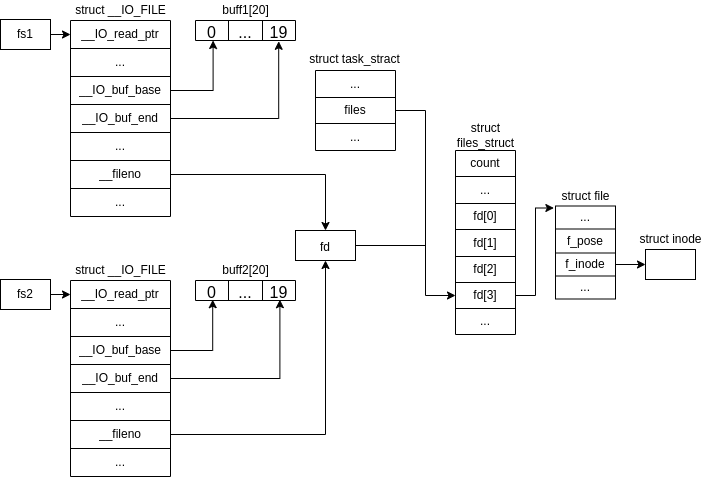
\includegraphics[scale=0.67]{assets/dCIO.png}
	\end{center}
	\caption{Схема структур программы}
\end{figure}

Функция open() создает файловый дескриптор для файла alphabet.txt в системной таблице открытых файлов. Далее функция fdopen() создает экземпляр структуры \_\_IO\_FILE при каждом вызове, поле \_\_fileno инициализируется значением дескриптора fd, возвращенного функцией open(). Функция setvbuf() явно задает размер буфера в 20 байт.

Первый fscanf() в цикле последовательно заполнит buff1 первыми 20 символами алфавита, при этом значение поля f\_pose в структуре struct file увеличится на 20. Второй вызов fscanf() в цикле последовательно заполнит buff2 оставшимися 6 символами (начиная с f\_pos = 20). Далее в цикле поочередно будут выводиться символы из buff1 и buff2.

\newpage
\begin{lstlisting}[caption=Исходная программа]
#include <stdio.h>
#include <fcntl.h>

int main()
{
	int fd = open("alphabet.txt",O_RDONLY);
	
	FILE *fs1 = fdopen(fd,"r");
	char buff1[20];
	setvbuf(fs1,buff1,_IOFBF,20);
	
	FILE *fs2 = fdopen(fd,"r");
	char buff2[20];
	setvbuf(fs2,buff2,_IOFBF,20);
	
	int flag1 = 1, flag2 = 2;
	while(flag1 == 1 || flag2 == 1)
	{
		char c;
		flag1 = fscanf(fs1,"%c",&c);
		if (flag1 == 1) {
			fprintf(stdout,"%c",c);
		}
		flag2 = fscanf(fs2,"%c",&c);
		if (flag2 == 1) { 
			fprintf(stdout,"%c",c); 
		}
	}
	return 0;
}
\end{lstlisting}

\begin{figure}[H]
	\begin{center}
		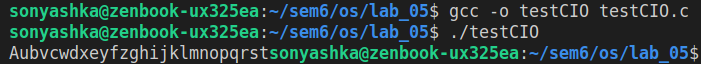
\includegraphics[scale=0.67]{assets/testCIO.png}
	\end{center}
	\caption{Результат работы}
\end{figure}

В случае многопоточной реализации и механизма взаимоисключения дополнительный поток получит доступ к данным только тогда, когда главный поток прочитает файл до конца, т.е. f\_pos = 26. Эту ситуацию можно разрешить создав два экземпляра дескрипторов открытых файлов.

\newpage
\begin{lstlisting}[caption=Программа с дополнительным потоком]
#include <stdio.h>
#include <fcntl.h>
#include <pthread.h>

typedef struct thread_args
{
	FILE *f;
	pthread_mutex_t *mutex;
} thread_args_t;

void run_thread(thread_args_t *args)
{
	pthread_mutex_lock(args->mutex);
	printf("\nThread 2: ");
	int flag = 1;
	while (flag == 1)
	{
		char c;
		flag = fscanf(args->f,"%c",&c);
		if (flag == 1) 
		{
			fprintf(stdout,"%c",c);
		}
	}
	pthread_mutex_unlock(args->mutex);
}

int main()
{
	setbuf(stdout, NULL);
	pthread_t thread;
	int fd = open("alphabet.txt",O_RDONLY);
	
	FILE *fs1 = fdopen(fd,"r");
	char buff1[20];
	setvbuf(fs1,buff1,_IOFBF,20);
	
	FILE *fs2 = fdopen(fd,"r");
	char buff2[20];
	setvbuf(fs2,buff2,_IOFBF,20);
	
	pthread_mutex_t mutex;
	pthread_mutex_init(&mutex, NULL);
	
	thread_args_t args;
	args.f = fs2;
	args.mutex = &mutex;
	pthread_create(&thread, NULL, run_thread, &args);
	
	pthread_mutex_lock(&mutex);
	printf("Thread 1: ");
	int flag = 1;
	while(flag == 1)
	{
		char c;
		flag = fscanf(fs1,"%c",&c);
		if (flag == 1) 
		{
			fprintf(stdout,"%c",c);
		}
	}
	pthread_mutex_unlock(&mutex);
	pthread_join(thread, NULL);
	pthread_mutex_destroy(&mutex);
	return 0;
}
\end{lstlisting}

\begin{figure}[H]
	\begin{center}
		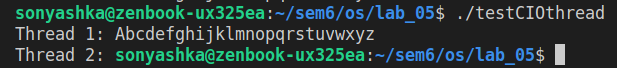
\includegraphics[scale=0.7]{assets/testCIOthread.png}
	\end{center}
	\caption{Результат работы}
\end{figure}

\chapter{Программа №2}

\begin{figure}[H]
	\begin{center}
		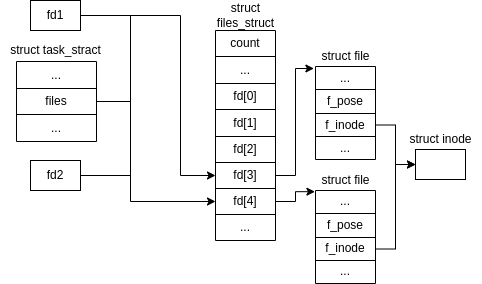
\includegraphics[scale=0.77]{assets/dKernelIO.png}
	\end{center}
	\caption{Схема структур программы}
\end{figure}

Каждый вызов функции open() создает дескриптор открытого файла в системной таблице открытых файлов, ссылающихся на один inode. Для каждого экземпляра struct file значение поля f\_pose меняется независимо, что позволяет избежать пропуска данных при чтении, используя разные дескрипторы.

\begin{lstlisting}[caption=Исходная программа]
#include <fcntl.h>
int main()
{
	char c;
	int fd1 = open("alphabet.txt",O_RDONLY);
	int fd2 = open("alphabet.txt",O_RDONLY);
	int rc1 = 1, rc2 = 1;
	while (rc1 == 1 && rc2 == 1)
	{
		if ((rc1 = read(fd1,&c,1)) == 1)
			write(1,&c,1);
		if ((rc2 = read(fd2,&c,1)) == 1)
			write(1,&c,1);
	}
return 0;
}
\end{lstlisting}

\begin{figure}[H]
	\begin{center}
		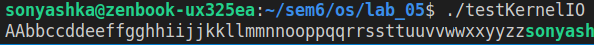
\includegraphics[scale=0.7]{assets/testKernelIO.png}
	\end{center}
	\caption{Результат работы}
\end{figure}

\begin{lstlisting}[caption=Программа с дополнительным потоком]
#include <stdio.h>
#include <fcntl.h>
#include <pthread.h>

typedef struct thread_args
{
	int *fd;
	pthread_mutex_t *mutex;
} thread_args_t;

void run_thread(thread_args_t *args)
{
	pthread_mutex_lock(args->mutex);
	char c;
	int rc = 1;
	while (rc == 1)
	{
		if ((rc = read(args->fd,&c,1)) == 1)
			write(1,&c,1);
	}
	pthread_mutex_unlock(args->mutex);
}

int main()
{
	char c;    
	pthread_t thread;
	int fd1 = open("alphabet.txt",O_RDONLY);
	int fd2 = open("alphabet.txt",O_RDONLY);
	pthread_mutex_t mutex;
	pthread_mutex_init(&mutex, NULL);
	
	thread_args_t args;
	args.fd = fd2;
	args.mutex = &mutex;
	pthread_create(&thread, NULL, run_thread, &args);
	pthread_mutex_lock(&mutex);
	int rc = 1;
	while (rc == 1)
	{
		if ((rc = read(fd1,&c,1)) == 1)
			write(1,&c,1);
	}
	pthread_mutex_unlock(&mutex);
	pthread_join(thread, NULL);
	pthread_mutex_destroy(&mutex);
	return 0;
}
\end{lstlisting}

\begin{figure}[H]
	\begin{center}
		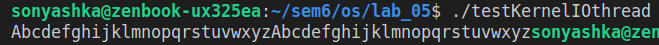
\includegraphics[scale=0.7]{assets/testKernelIOthread.png}
	\end{center}
	\caption{Результат работы}
\end{figure}

\chapter{Программа №3}

\begin{figure}[H]
	\begin{center}
		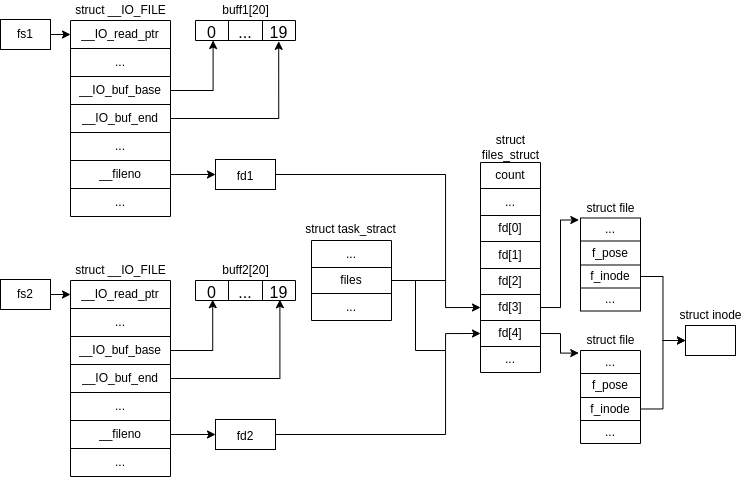
\includegraphics[scale=0.65]{assets/dtest.png}
	\end{center}
	\caption{Схема структур программы}
\end{figure}

Файл открывается два раза на запись с использованием функции fopen(), т.е. создается два экземпляра структуры \_\_IO\_FILE, каждому соответствует дескриптор открытого файла в системной таблице открытых файлов. 

Функция fprintf() предосставляет буферизованный вывод. Информация будет записываться в буфер до тех пор, пока либо не переполнится буфер, либо не будут вызваны fflush() или fclose(). В случае программы ниже, запись произведется при вызове fclose(). Так как для каждого экземпляра созданы отдельные экземпляры struct file, то и значения полей f\_pose будут изменятся независимо для каждого файла. 

При первом вызове fclose() информация будет записана в файл. При следующем вызове fclose() данные записываются с начала файла, а предыдущая информация теряется. Данная проблема может быть решена использованием одного неделимого системного вызова O\_APPEND. В таком случае запись запись будет производиться в конец файла.

Также функция fopen() в качестве флагов принимает const char *mode, в соответствии с которыми устанавливаются флаги для вызова open().

\begin{lstlisting}[caption=Исходная программа]
#include <stdio.h>
#include <fcntl.h>
#define FILE_NAME "out.txt"

int main()
{
	struct stat st1, st2;
	FILE *f1 = fopen(FILE_NAME, "w");
	stat(FILE_NAME, &st1);
	printf("F1 OPEN: inode = %d, size = %d\n", st1.st_ino, st1.st_size);
	FILE *f2 = fopen(FILE_OPEN, "w");
	stat(FILE_NAME, &st2);
	printf("F2 OPEN: inode = %d, size = %d\n", st2.st_ino, st2.st_size);
	
	for (char c = 'a'; c <= 'z'; c++)
	{
		if (c % 2)
			fprintf(f1, "%c", c);
		else
			fprintf(f2, "%c", c);
	}
	fclose(f1);
	stat(FILE_NAME, &st1);
	printf("F1 CLOSE: inode = %d, size = %d\n", st1.st_ino, st1.st_size);
	fclose(f2);
	stat(FILE_NAME, &st2);
	printf("F2 CLOSE: inode = %d, size = %d\n", st2.st_ino, st2.st_size);
	return 0;
}
\end{lstlisting}

\begin{figure}[H]
	\begin{center}
		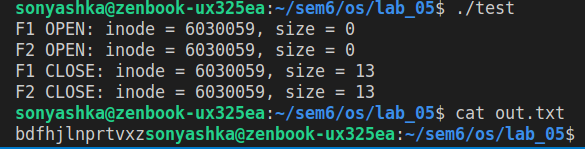
\includegraphics[scale=0.7]{assets/test.png}
	\end{center}
	\caption{Результат работы}
\end{figure}
\newpage
\begin{lstlisting}[caption=Программа с дополнительным потоком]
#include <stdio.h>
#include <fcntl.h>
#include <sys/stat.h>
#include <pthread.h>
#define FILE_NAME "outThread.txt"

void run_thread(FILE *f)
{
	for (char c = 'b'; c <= 'z'; c += 2)
	{
		fprintf(f, "%c", c);
	}
}

int main()
{
	pthread_t thread;
	struct stat st1, st2;
	FILE *f1 = fopen(FILE_NAME, "w");
	stat(FILE_NAME, &st1);
	printf("F1 OPEN: inode = %d, size = %d\n", st1.st_ino, st1.st_size);
	FILE *f2 = fopen(FILE_NAME, "w");
	stat(FILE_NAME, &st2);
	printf("F2 OPEN: inode = %d, size = %d\n", st2.st_ino, st2.st_size);
	
	pthread_create(&thread, NULL, run_thread, f2);
	for (char c = 'a'; c <= 'z'; c += 2)
	{
		fprintf(f1, "%c", c);
	}
	
	pthread_join(thread, NULL);
	fclose(f1);
	stat(FILE_NAME, &st1);
	printf("F1 CLOSE: inode = %d, size = %d\n", st1.st_ino, st1.st_size);
	fclose(f2);
	stat(FILE_NAME, &st2);
	printf("F2 CLOSE: inode = %d, size = %d\n", st2.st_ino, st2.st_size);
	return 0;
}
\end{lstlisting}

\begin{figure}[H]
	\begin{center}
		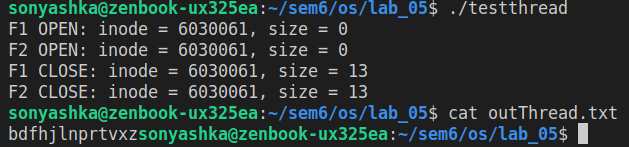
\includegraphics[scale=0.7]{assets/testThread.png}
	\end{center}
	\caption{Результат работы}
\end{figure}

Ниже представлены листинги структур struct stat и struct \_\_IO\_FILE.

\begin{lstlisting}[caption=struct stat]
struct stat {
	dev_t         st_dev;      /* device */
	ino_t         st_ino;      /* inode */
	mode_t        st_mode;     /* access mode */
	nlink_t       st_nlink;    /* number of hardlink */
	uid_t         st_uid;      /* user id */
	gid_t         st_gid;      /* group id */
	dev_t         st_rdev;     /* device type */
	/* (if its a device) */
	off_t         st_size;     /* size in bytes */
	blksize_t     st_blksize;  /* size of IO-block */
	/* in FS */
	blkcnt_t      st_blocks;   /* count of allocated blocks */
	time_t        st_atime;    /* time of last access */
	time_t        st_mtime;    /* time of last modification */
	time_t        st_ctime;    /* time of last changing */
};
\end{lstlisting}

\begin{lstlisting}[caption=struct \_\_IO\_FILE]
struct _IO_FILE
{
	int _flags;         /* High-order word is _IO_MAGIC; rest is flags. */
	/* The following pointers correspond to the C++ streambuf protocol. */
	char *_IO_read_ptr;        /* Current read pointer */
	char *_IO_read_end;        /* End of get area. */
	char *_IO_read_base;        /* Start of putback+get area. */
	char *_IO_write_base;        /* Start of put area. */
	char *_IO_write_ptr;        /* Current put pointer. */
	char *_IO_write_end;        /* End of put area. */
	char *_IO_buf_base;        /* Start of reserve area. */
	char *_IO_buf_end;        /* End of reserve area. */
	/* The following fields are used to support backing up and undo. */
	char *_IO_save_base; /* Pointer to start of non-current get area. */
	char *_IO_backup_base;/*Pointer to firstvalid character of backuparea*/
	char *_IO_save_end; /* Pointer to end of non-current get area. */
	struct _IO_marker *_markers;
	struct _IO_FILE *_chain;
	int _fileno;
	int _flags2;
	__off_t _old_offset; /* This used to be _offset but it's too small.  */
	/* 1+column number of pbase(); 0 is unknown. */
	unsigned short _cur_column;
	signed char _vtable_offset;
	char _shortbuf[1];
	_IO_lock_t *_lock;
	#ifdef _IO_USE_OLD_IO_FILE
};
\end{lstlisting}

\end{document}